%% LaTeX Beamer presentation template (requires beamer package)
%% see http://latex-beamer.sourceforge.net/
%% idea contributed by H. Turgut Uyar
%% template based on a template by Till Tantau
%% this template is still evolving - it might differ in future releases!

\documentclass{beamer}

\mode<presentation>
{
\usetheme{Darmstadt}
\setbeamertemplate{navigation symbols}{} 
\setbeamercovered{dynamic}
}

\usepackage[brazil]{babel}
\usepackage[utf8]{inputenc}
\usepackage{mathptmx}% font definitions, try \usepackage{ae} instead of the following
\usepackage[scaled=.90]{helvet}% three lines if you don't like this look
\usepackage{courier}
\usepackage[T1]{fontenc}
\usepackage{algorithmic}
\usepackage{url}

\title{Algoritmos de Roteamento}

%\subtitle{}

% - Use the \inst{?} command only if the authors have different
%   affiliation.
%\author{F.~Author\inst{1} \and S.~Another\inst{2}}
\author{Pedro Paulo V. Campos \\ Tarcísio Eduardo M. Crocomo}

\date{\today}


% This is only inserted into the PDF information catalog. Can be left
% out.
\subject{Algoritmos de Roteamento}



% If you have a file called "university-logo-filename.xxx", where xxx
% is a graphic format that can be processed by latex or pdflatex,
% resp., then you can add a logo as follows:

% \pgfdeclareimage[height=0.5cm]{university-logo}{university-logo-filename}
% \logo{\pgfuseimage{university-logo}}



% Delete this, if you do not want the table of contents to pop up at
% the beginning of each subsection:
\AtBeginSection[]
{
\begin{frame}<beamer>
\frametitle{Sumário}
\tableofcontents[currentsection,currentsubsection]
\end{frame}
}

% If you wish to uncover everything in a step-wise fashion, uncomment
% the following command:

%\beamerdefaultoverlayspecification{<+->}

\begin{document}

\begin{frame}
\titlepage
\end{frame}

\begin{frame}
\frametitle{Sumário}
\tableofcontents
% You might wish to add the option [pausesections]
\end{frame}


\section{Introdução}
\subsection{}

\begin{frame}
\frametitle{Motivação}
\texttt{\footnotesize traceroute to \textbf{nhk.co.jp} (61.58.37.103) \\
 1  192.168.1.254  0.150 ms \\
 2  \textbf{roteador.inf.ufsc.br}  1.835 ms \\
 3  npd252e1-1gb-\textbf{npd}254rs.bb.ufsc.br  5.233 ms \\
 4  popsc-1g-ufsc-(...)-r250.bb.\textbf{pop-sc}.rnp.br  5.939 ms \\
 5  rnp-2g-194-251-v40-r251.bb.pop-sc.rnp.br  6.613 ms \\
 6  so-1-0-0-r1-\textbf{rs}.bkb.rnp.br  11.776 ms \\
 7  so-0-0-0-r1-\textbf{df}.bkb.rnp.br  51.419 ms \\
 8  so-0-2-0-r1-\textbf{sp}.bkb.rnp.br  66.531 ms \\
(...) \\
16  xe-0-1-0.r21.\textbf{miam}fl02.us.bb.gin.ntt.net 177.438 ms \\
(...) \\
20  as-1.r21.\textbf{osak}jp01.jp.bb.gin.ntt.net  396.762 ms \\
21  ae-2.r23.\textbf{toky}jp01.jp.bb.gin.ntt.net  374.946 ms \\
22  129.250.3.75  407.060 ms \\
23  xe-1-1-0.a05.\textbf{taip}tw01.tw.ra.gin.ntt.net 430.482 ms \\
(...) \\
27  nhk-grp.\textbf{jp}  408.878 ms
}
\end{frame}

\begin{frame}
\frametitle{O Roteador}
%\usepackage{graphics} is needed for \includegraphics
\begin{figure}[htp]
\begin{center}
  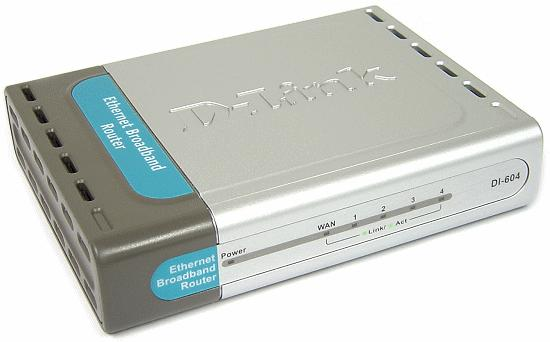
\includegraphics[width=90mm]{Imagens/D-Link.jpg}
  \caption[dlink]{DI-604: 100 Mbps, \$60}
  \label{dlink}
\end{center}
\end{figure}
\end{frame}

\begin{frame}
\frametitle{O Roteador}
%\usepackage{graphics} is needed for \includegraphics
\begin{figure}[htp]
\begin{center}
  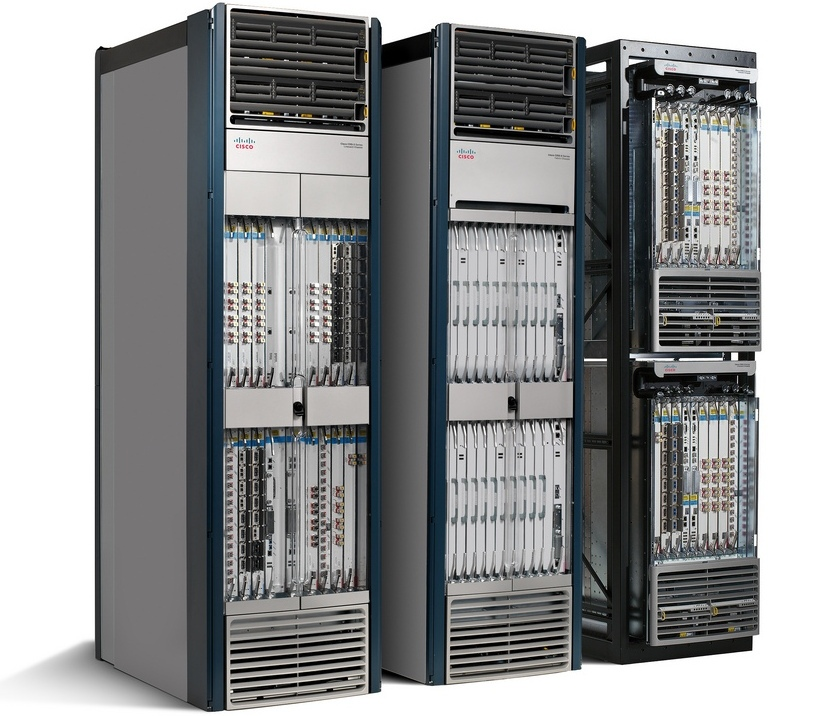
\includegraphics[width=73mm]{Imagens/Cisco-CRS-3.jpeg}
  \caption[cisco]{Cisco CRS-3: 322 Tbps, \$60.000}
  \label{cisco}
\end{center}
\end{figure}
\end{frame}

\begin{frame}
\frametitle{Desafios}
\begin{description}
  \setlength{\itemsep}{0.7cm}%
  \item[Correção] Fornecer não apenas uma rota válida mas a melhor
  \item[Escalabilidade] Tamanho de rede variável. Algoritmos
  eficientes
  \item[Estabilidade] Rápida adaptação a mudanças ou problemas na rede
  \item[Robustez] Funcionar por anos sem necessitar reinicialização
  \item[Justiça] Visar eficiência global sem gerar starvation
\end{description}

\end{frame}


\section{Fundamentação}
\subsection{}

\begin{frame}
\frametitle{Modelos de troca de dados}
 	
\end{frame}

\begin{frame}
\frametitle{Métricas para classificação de rotas}
\begin{itemize}
  \setlength{\itemsep}{0.7cm}%
  \item Número de hops
  \item Largura de banda
  \item Custo (monetário)
\end{itemize}
\end{frame}

\begin{frame}
\frametitle{Sistemas Autônomos}
\begin{itemize}
  \setlength{\itemsep}{0.7cm}%
  \item Como tornar escalável e administrável um conjunto de \textasciitilde2bi de
  computadores interconectados?
  \item Solução: Agrupar em um SA redes operadas por um ou mais operadores que apresentam uma única política clara de roteamento.
  \item Exemplo: AS11242 - POP-SC - Responsável por 73728 IPs 
\end{itemize}
\end{frame}

\begin{frame}
\frametitle{Classificação de protocolos de roteamento}
\framesubtitle{Quanto à vizinhança}
\begin{block}{Externos}
G(V,A)\\
V = \{v $\mid$ v  é um sistema autônomo\}\\
A = \{($v_1$, $v_2$, m) $\mid$ $v_1$, $v_2 \in$ V, há uma ligação direta
entre $v_1$ e $v_2$  com um custo m\}
\end{block}

\begin{block}{Internos}
G(V,A)\\
V = \{v $\mid$ v é nodo da rede de um sistema autônomo\}\\
A = \{($v_1$, $v_2$, m) $\mid$ $v_1$, $v_2 \in$ V, há uma ligação direta
entre $v_1$ e $v_2$  com um custo m\}
\end{block}
\end{frame}

\begin{frame}
\frametitle{Classificação de protocolos de roteamento}
\framesubtitle{Quanto à vizinhança}
%\usepackage{graphics} is needed for \includegraphics
\begin{figure}[htp]
\begin{center}
  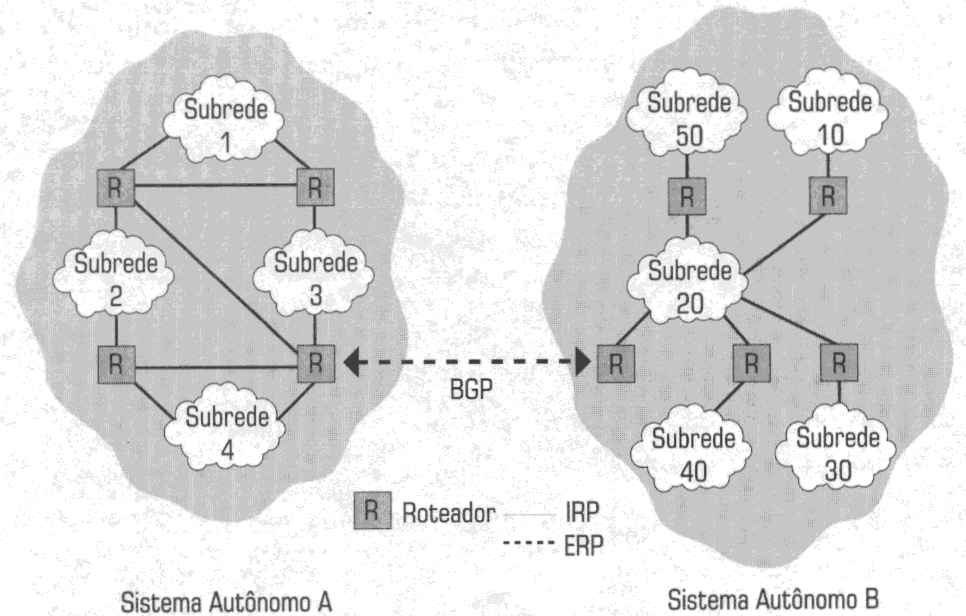
\includegraphics[width=105mm]{Imagens/SistemaAutonomo.png}
  \label{sistema_autonomo}
\end{center}
\end{figure}
\end{frame}

\begin{frame}
\frametitle{Classificação de protocolos de roteamento}
\framesubtitle{Quanto à escolha de rotas}
\begin{itemize}
  \item Estáticos (Não adaptativos)
  \begin{itemize}
     \item Menor caminho
     \item \emph{Flooding}
     \item Baseado em Fluxo (\emph{Flow-based}) 
  \end{itemize}
  \item Dinâmicos (Adaptativos)
  \begin{itemize}
     \item Vetor distância
     \item Estado do enlace (\emph{Link State})
     \item Hierárquico 
  \end{itemize}
\end{itemize}

\end{frame}

\begin{frame}
\frametitle{Rotas Ótimas}
\begin{itemize}
  \setlength{\itemsep}{0.7cm}%
  \item É possível criar uma descrição das rotas ótimas sem levar em conta a
  topologia da rede?
  \item Como medir a qualidade de um algoritmo de roteamento?
\end{itemize}
\end{frame}

\begin{frame}
\frametitle{Princípio de otimização}
\begin{block}{Teorema}
Se um roteador \emph{J} estiver no caminho ótimo entre os roteadores \emph{I} e \emph{K}, o caminho
ótimo de \emph{J} a \emph{K} também estará na mesma rota.
\end{block}
%\usepackage{graphics} is needed for \includegraphics
\begin{figure}[htp]
\begin{center}
  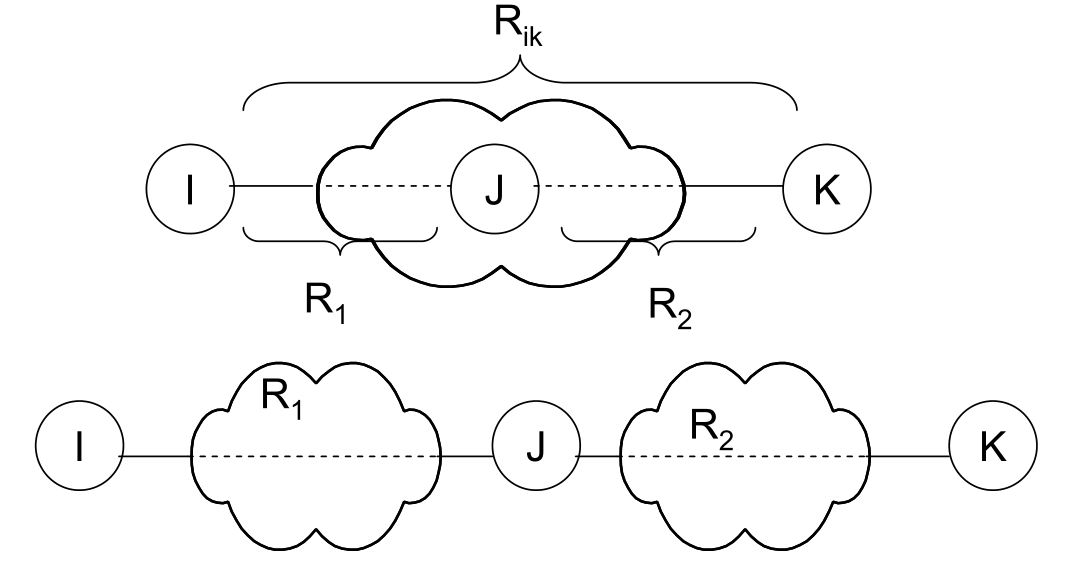
\includegraphics[width=80mm]{Imagens/PrincipioOtimizacao.jpeg}
  \label{principio_otimizacao}
\end{center}
\end{figure}
\end{frame}

\begin{frame}
\frametitle{Princípio de otimização}
\begin{block}{Prova (por contradição)}
Se houvesse uma rota melhor que a enunciada entre \emph{J} e \emph{K}, ela poderia ser
concatenada a $R_1$ para criar uma rota melhor entre \emph{I} e \emph{K}, contradizendo a
afirmação que a rota $R_{ik}$ é ótima.
\end{block}
%\usepackage{graphics} is needed for \includegraphics
\begin{figure}[htp]
\begin{center}
  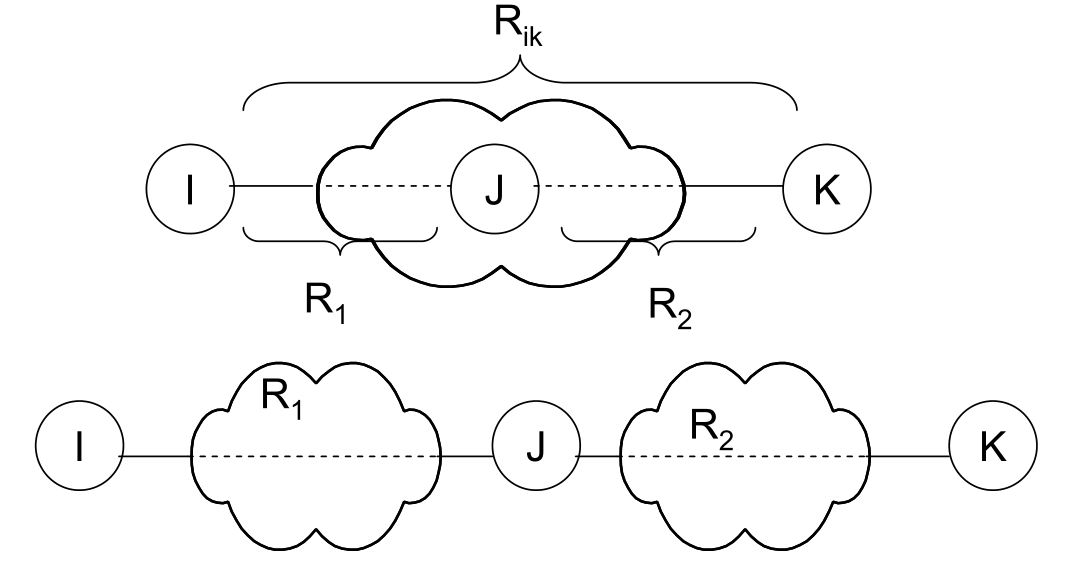
\includegraphics[width=80mm]{Imagens/PrincipioOtimizacao.jpeg}
  \label{principio_otimizacao2}
\end{center}
\end{figure}
\end{frame}

\begin{frame}
\frametitle{Árvore de Escoamento}
%\usepackage{graphics} is needed for \includegraphics
\begin{figure}[htp]
\begin{center}
  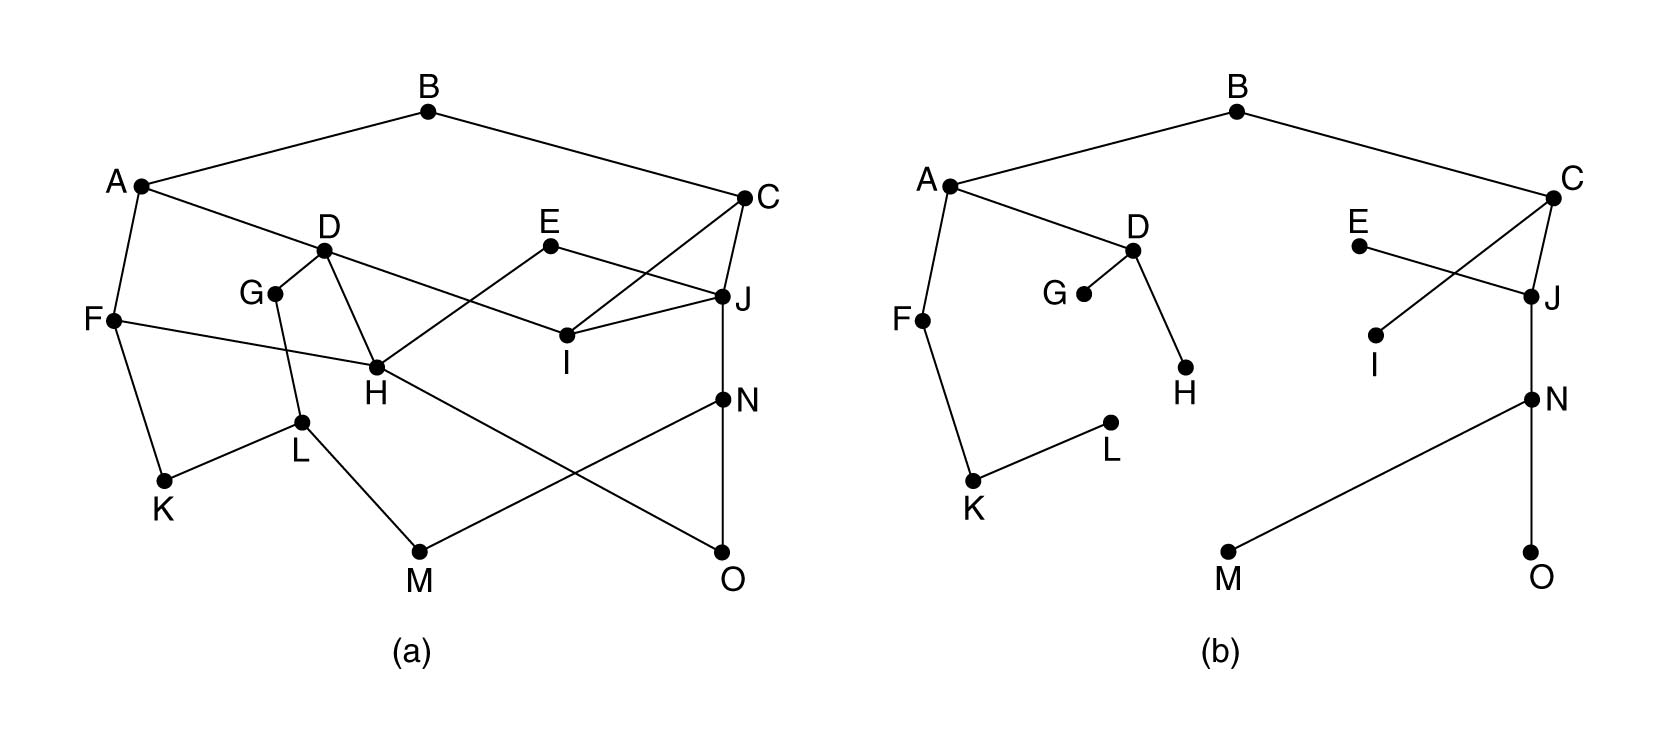
\includegraphics[width=108mm]{Imagens/ArvoreEscoamento.jpeg}
  \label{arvore_escoamento}
\end{center}
\end{figure}
\end{frame}


\section{Algoritmos Estáticos}
\subsection{}

\begin{frame}
\frametitle{Menor Caminho}

\begin{itemize}
  \setlength{\itemsep}{0.7cm}%
  \item Um dos algoritmos mais simples
  \item A partir do modelo de grafos de uma rede interna gera uma sequência de
  nodos a serem percorridos para um pacote sair da origem e chegar ao destino.
  \item Algoritmo global, conhecimento completo do grafo 
  \item Calculado de maneira centralizada e distribuída para os roteadores
  \item Algoritmo de Dijkstra
\end{itemize}
\end{frame}

\begin{frame}
\frametitle{\emph{Flooding}}

\begin{itemize}
  \setlength{\itemsep}{0.7cm}%
  \item Envia pacotes para todos os vizinhos, exceto pra de onde ele veio
  \item Necessita de controle para evitar o envio de infinitos pacotes
  \item Não costuma ser prático, exceto quando seu efeito é efetivamente o desejado
  \item Escolhe o menor caminho, pois escolhe todos simultaneamente 
\end{itemize}
\end{frame}

\begin{frame}
\frametitle{Baseado em Fluxo}
\begin{itemize}
  \setlength{\itemsep}{0.7cm}%
  \item Conta carga da rede junto da topologia
  \item Fluxo médio conhecido anteriormente
  \item Cálculo do atraso médio entre nodos
  \item Algoritmo que determine menor atraso médio determina o roteamento
\end{itemize}
\end{frame}


\section{Algoritmos Dinâmicos}
\subsection{}

\begin{frame}
\frametitle{Vetor Distância}
\begin{itemize}
  \setlength{\itemsep}{0.7cm}%
  \item Algoritmo distribuído
  \item Cada roteador possui uma tabela (vetor) contendo a melhor distância conhecida até cada destino e a linha de saída preferencial utilizada para alcançá-lo.
  \item Utilizado na ARPANET: \emph{Routing Information Protocol} (RIP)
  \item Objetivo: Encontrar o menor caminho
  \begin{itemize}
    \item Algoritmo de Bellman-Ford
  \end{itemize}
\end{itemize}
\end{frame}

\begin{frame}
\frametitle{Algoritmo de Bellman-Ford}
\begin{block}{Princípio}
Se os vizinhos de um nodo \emph{i} conhecem um caminho até um nodo \emph{j}, a menor distância
entre o nodo \emph{i} e \emph{j} é obtido encontrando o menor valor resultante
da soma da distância de \emph{i} até um vizinho e deste até \emph{j}.
\end{block}
%\usepackage{graphics} is needed for \includegraphics
\begin{figure}[htp]
\begin{center}
  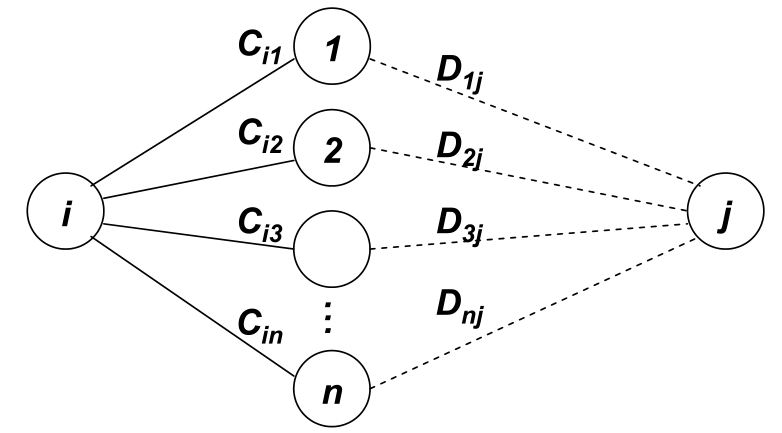
\includegraphics[width=85mm]{Imagens/BellmanFord.jpeg}
  \label{bellman_ford}
\end{center}
\end{figure}
\end{frame}

\begin{frame}
\begin{block}{Algoritmo}
\begin{algorithmic}
    \STATE Bellman-Ford(G, w, s)
    \FOR{i $\gets$ 1 to $\mid$V[G]$\mid$ - 1}
    	\FORALL{(u, v) $\gets$ E[G]}
    		\STATE Relax(u, v)
    	\ENDFOR
    \ENDFOR 
    \FORALL{(u, v) $\gets$ E[G]}
    	\IF{d[v] > d[u] + w(u, v)}
    		\RETURN FALSE
    	\ENDIF
   	\ENDFOR
   	\RETURN TRUE
\end{algorithmic}
\end{block}
\end{frame}

\begin{frame}
\frametitle{Vetor Distância}
%\usepackage{graphics} is needed for \includegraphics
\begin{figure}[htp]
\begin{center}
  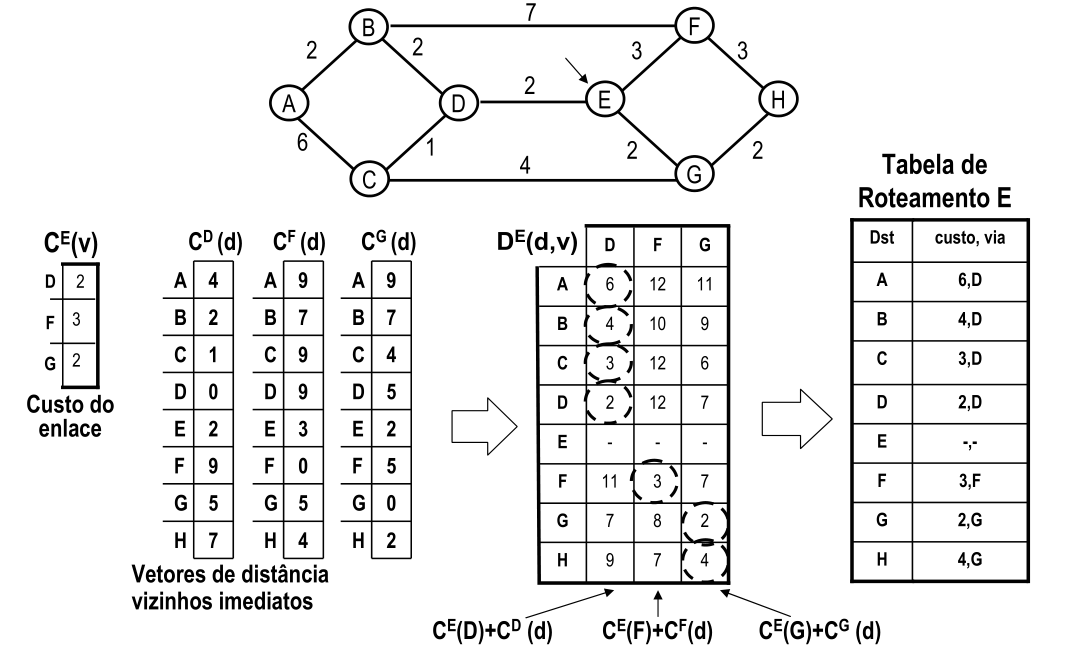
\includegraphics[width=105mm]{Imagens/VetorDistancia.png}
  \label{vetor_distancia}
\end{center}
\end{figure}
\end{frame}

\begin{frame}
\frametitle{Convergência do Vetor Distância}

\begin{itemize}
  \item Vetor distância reage bem (linearmente) a boas notícias:
  %\usepackage{graphics} is needed for \includegraphics
\begin{figure}[htp]
\begin{center}
  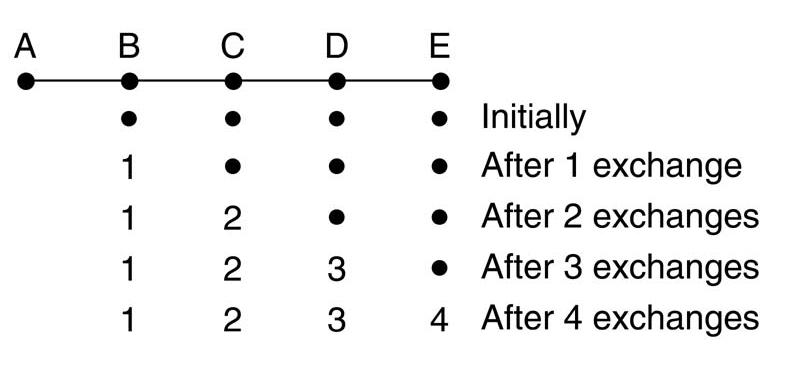
\includegraphics[width=85mm]{Imagens/ConvergenciaVetorDistancia.jpeg}
  \label{convergencia_vetor_distancia}
\end{center}
\end{figure}
   \item Já a más notícias\ldots
\end{itemize}
\end{frame}

\begin{frame}
\frametitle{Problema da Contagem ao Infinito}
 %\usepackage{graphics} is needed for \includegraphics
\begin{figure}[htp]
\begin{center}
  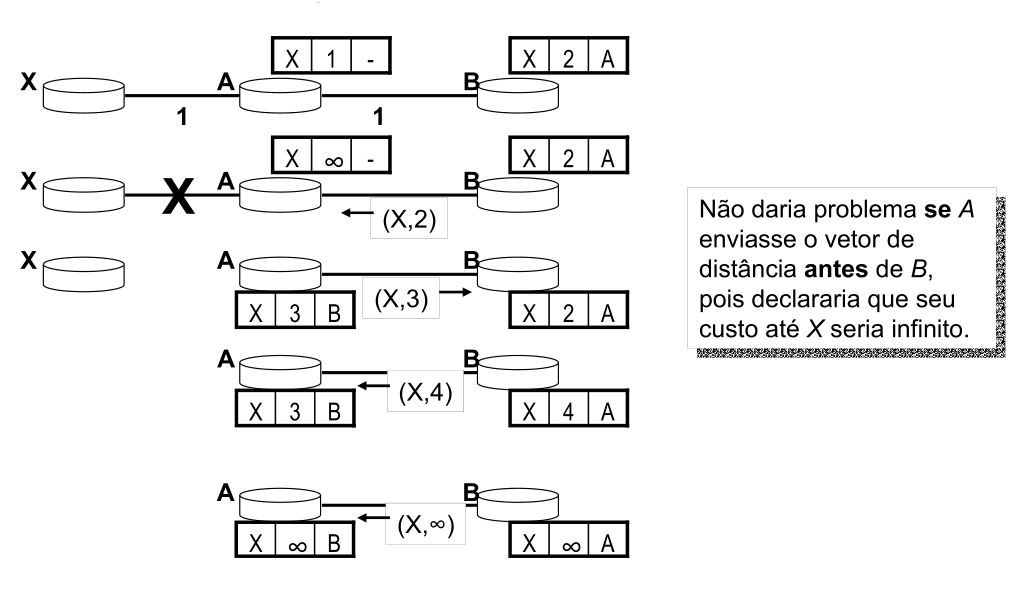
\includegraphics[width=105mm]{Imagens/ContagemAoInfinito.jpeg}
  \label{contagem_ao_infinito}
\end{center}
\end{figure}
\end{frame}

\begin{frame}
\frametitle{Estado do link}

\begin{itemize}
  \item Descobrir vizinhos
  \item Propagar informação
  \begin{itemize}
     \item Quem
     \item Vizinhos
     \item Número de sequência
  \end{itemize}
  \item Criação do mapa da rede
  \item Recalcular e reenviar em caso de falha
  \item Cálculo da melhor rota é independente
  \item OSPF - Open Shortest Path First:
  \begin{itemize}
     \item Protocolo muito utilizado em redes internas,
        baseado em link-state.
  \end{itemize}
\end{itemize}
\end{frame}

\begin{frame}
\frametitle{Roteamento hierárquico}
\begin{itemize}
  \setlength{\itemsep}{0.7cm}%
  \item Utilizado no roteamento externo (inter-rede)
  \item \textasciitilde2bi de dispositivos $\to$ 35.000 Sistemas Autônomos
  (2010)
  \item Exemplo: Border Gateway Protocol (BGP)
  \item Responsável por tornar a Internet uma aplicação verdadeiramente distribuída.
  \item Obediência a leis internacionais e decisões políticas
\end{itemize}
\end{frame}

\begin{frame}
\frametitle{Roteamento Hierárquico}
\begin{itemize}
  \item Funcionamento básico: Similar ao vetor distância. Roteadores enviam uns
  aos outros duas informações:
  \begin{itemize}
    \item Que eles estão vivos e quais redes (Faixas de IPs) estão sob sua
    responsabilidade.
    \item Qual a rota completa que utilizam para chegar ao destino (Solução para
    o problema da contagem ao infinito!)
  \end{itemize}
\end{itemize}
\end{frame}

\begin{frame}
\frametitle{Roteamento Hierárquico}
 %\usepackage{graphics} is needed for \includegraphics
\begin{figure}[htp]
\begin{center}
  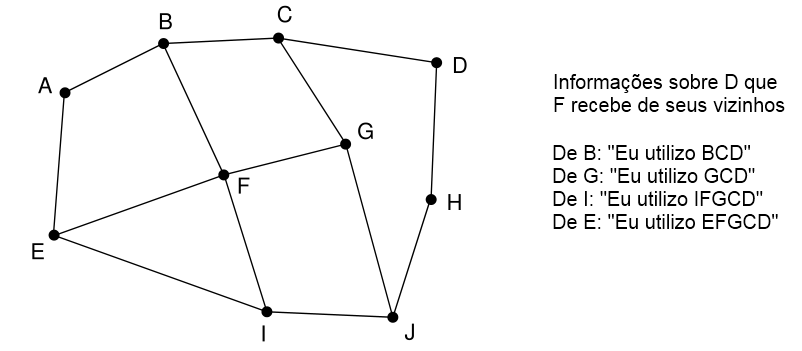
\includegraphics[width=100mm]{Imagens/RoteamentoHierarquico.png}
  \label{roteamento_hierarquico}
\end{center}
\end{figure}
\begin{itemize}
  \item O que acontece se G cair?
\end{itemize}
\end{frame}


\section{Conclusão}
\subsection{}

\begin{frame}
\frametitle{Conclusão}
\begin{itemize}
  \setlength{\itemsep}{0.7cm}%
  \item Grafos e seus algoritmos são ferramentas extremamente úteis em redes de
  computadores. Permitem a modelagem e solução de diferentes situações encontradas na área.
  \item A Internet como a conhecemos só existe hoje graças aos avanços no
  desenvolvimento de melhores e mais eficientes algoritmos de roteamento.
  \item Não há uma "bala de prata", diferentes algoritmos servem a diferentes
  propósitos
\end{itemize}
\end{frame}

\begin{frame}
\frametitle{Bibliografia}
\begin{itemize}
  \item TANENBAUM, A. S. Redes de Computadores. 4 ed. São Paulo: Elsevier, 2003.
  \item DE CASTRO, M. C. F. Redes Comutadas. setembro de 2002. Disponível em:
  <\url{http://www.ee.pucrs.br/~decastro/download.html}>.
  \item CARISSIMI, A. Algoritmos de roteamento. 2008. Disponível em:
  <\url{http://www.inf.ufrgs.br/~asc/redes/pdf/aula21.pdf}>.
  \item CAMPONOGARA, E. Caminhos Mínimos Com Uma Fonte. abril de 2009.
  Disponível em:
  <\url{http://www.das.ufsc.br/~camponog/Disciplinas/DAS-9003/slides_CLR/l14-shortest-path.pdf}>
\end{itemize}
\end{frame}

\end{document}
